\chapter{12-step Tutorial}

\section{Preconditions}
In order to perform this tutorial, install Kobold and start the Client, Server and
Server Administration Tool. Make sure that you have set the correct properties for your
Client. 


\section{Creating a productline}
In your SAT Tool, enter the command 'newpl'. A listing is shown with the properties of the lately created
productline. Enter the command '1' and then 'testproductline' as name for your
new productline. Enter the command 'p' to create the productline.

\begin{figure}[h!]
\begin{center}

\includegraphics[width=10cm]{tutorial1.png}
   \caption{Creating a productline}
\end{center}
\end{figure}\par


\section{Creating a new user}
In your SAT Tool, enter the command 'newuser'. A listing is shown with the properties of the lately created
user, his/her username, fullname and initial password. 
Enter the command '1' and then 'testuser' as username for your new user.
Enter the command 'p' to create the user.

\begin{figure}[h!]
\begin{center}

\includegraphics[width=10cm]{tutorial2.png}
   \caption{Creating a new user}
\end{center}
\end{figure}\par


\section{Assigning an existing user to a productline as PLE}
In your SAT Tool, enter the command 'assignple'. 
As PLE enter the username 'testuser'. As productline enter your productline 'testproductline'.

\begin{figure}[h!]
\begin{center}

\includegraphics[width=10cm]{tutorial3.png}
   \caption{Assigning your ple to your productline}
\end{center}
\end{figure}\par



\section{Starting a new project}

Start the Client.
In the File menu select 'New' and then 'Kobold PLAM Project'. The Kobold wizard opens.
Enter the url of your Kobold server, your username (testuser) and a blank for your password. Then press
"test connection". If the test succeeds, the "next" button is enabled.

\begin{figure}[h!]
\begin{center}
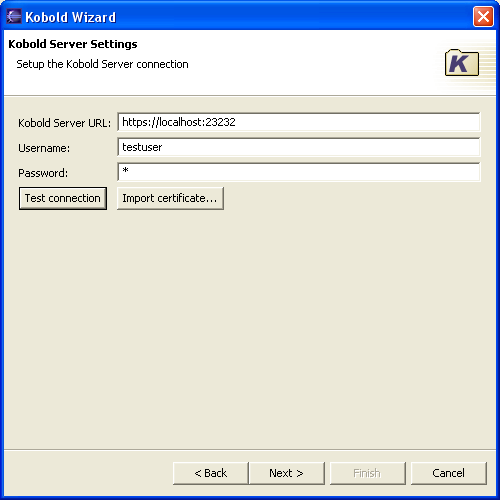
\includegraphics[width=10cm]{tutorial4.png}
   \caption{Kobold wizard}
\end{center}
\end{figure}\par

After that you choose 'testproductline' as the productline you want to check out.

\begin{figure}[h!]
\begin{center}
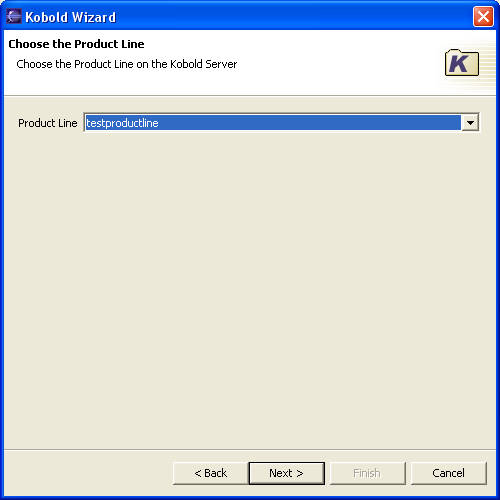
\includegraphics[width=10cm]{tutorial5.png}
   \caption{Kobold wizard}
\end{center}
\end{figure}\par

In the last step you have to enter 'testproject' as the name of the project you want to create.

\begin{figure}[h!]
\begin{center}
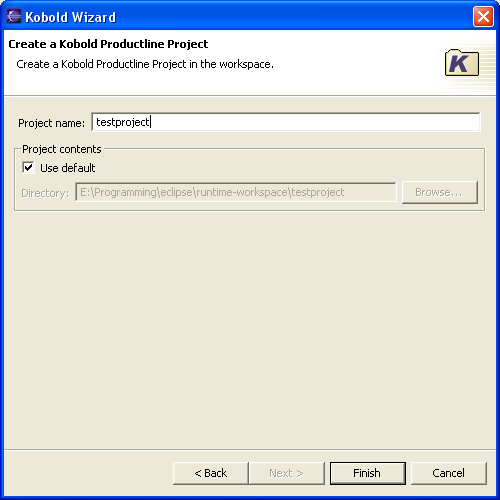
\includegraphics[width=10cm]{tutorial6.png}
   \caption{Kobold wizard}
\end{center}
\end{figure}\par

Press finish and your new project is created.


\section{Creating a Core Assets}

In the Architecture Tree (on the left) open up the tree of your new project. Double-click on 'architecture' in order to 
open the Architecture Editor. \par

Open the pallete on the right of the Architecture Editor and select the 'component' item. Click in 
the Architecture Editor. A core asset is inserted and a dialog opens where you enter 'componentA' as name of
the core asset. 

\begin{figure}[h!]
\begin{center}
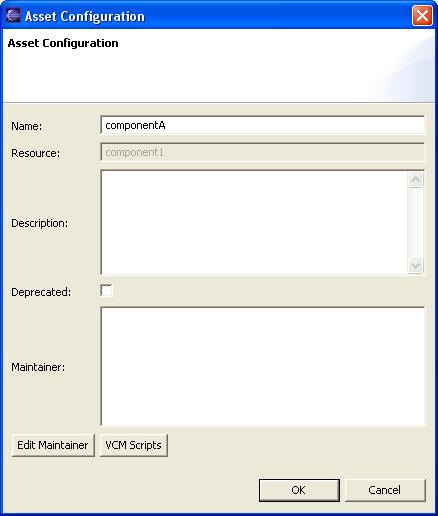
\includegraphics[width=8cm]{tutorial7.png}
   \caption{Asset Configuration Core Asset}
\end{center}
\end{figure}\par

Repeat these steps another two times and create the core assets 'componentB' and
'componentC'. After this your architecture should look like the following:

\begin{figure}[h!]
\begin{center}

\includegraphics[width=10cm]{tutorial8.png}
   \caption{Your Core Assets}
\end{center}
\end{figure}\par


\section{Creating variants}

In the pallete select the "variant" item. Click within componentA in 
the Architecture Editor. A variant is inserted and a dialog opens where you can enter 'variantA1' as name of
the variant. 

\begin{figure}[h!]
\begin{center}
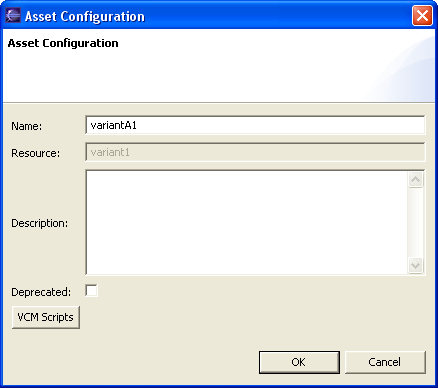
\includegraphics[width=10cm]{tutorial9.png}
   \caption{Asset Configuration Variant}
\end{center}
\end{figure}\par

Repeat these steps another two times in order to create the variants 'variantA2' and 'variantB'.
After this your architecture should look like the following:

\begin{figure}[h!]
\begin{center}

\includegraphics[width=10cm]{tutorial10.png}
   \caption{Your Variants}
\end{center}
\end{figure}\par


\section{Creating releases}

In the pallete select the "release" item. Click within variantA1 in 
the Architecture Editor. A release is inserted and a dialog opens where you can enter 'releaseA' as name of
the release. 

\begin{figure}[h!]
\begin{center}
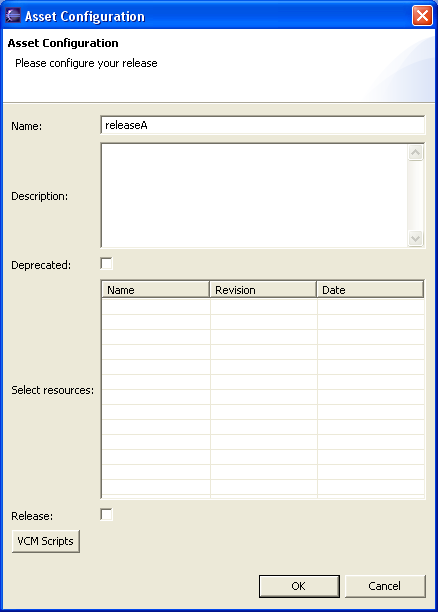
\includegraphics[width=10cm]{tutorial11.png}
   \caption{Asset Configuration Release}
\end{center}
\end{figure}\par

Repeat these steps another two times in order to create the releases 'releaseB1' and 
'releaseB2'. After this your architecture should look like the following:

\begin{figure}[h!]
\begin{center}

\includegraphics[width=10cm]{tutorial12.png}
   \caption{Your Releases}
\end{center}
\end{figure}\par



\section{Creating dependency edges}

In the pallete select the "include edge" item. Select the assets 'variantA1', 'releaseB1', 
'componentA' and 'componentC' in this order. Two dependency edges appear between the
assets. After this your architecture should look like the following:

\begin{figure}[h!]
\begin{center}

\includegraphics[width=10cm]{tutorial13.png}
   \caption{Dependency edges}
\end{center}
\end{figure}\par



\section{Creating a product}

In the palette press 'compose product'. The components, etc. in the architecture editor turn
grey. Select 'releaseA'. The chosen object and all the objects that are needed for it turn blue. 

\begin{figure}[h!]
\begin{center}

\includegraphics[width=10cm]{tutorial14.png}
   \caption{Creating a product - step 1}
\end{center}
\end{figure}\par


Press the 
'create product' button in the Architecture Editor. A dialog opens where you can enter 'testproduct' as
the name of your new product. After confirming the dialog, you can see
your new product in the Architecture Tree and Architecture Editor.

\begin{figure}[h!]
\begin{center}
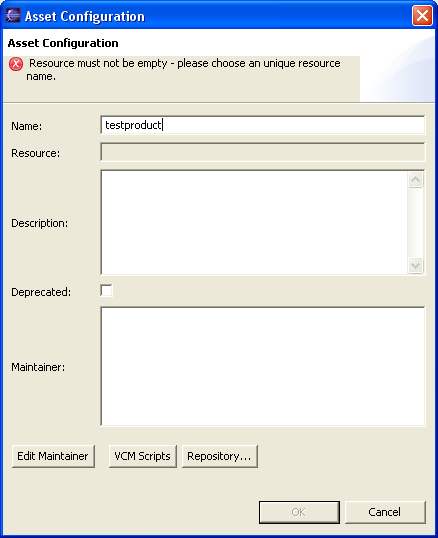
\includegraphics[width=10cm]{tutorial15.png}
   \caption{Creating a product - step 2}
\end{center}
\end{figure}\par





\section{Writing a mail}

In the menu of the Workflow View select "new mail". A Workflow window opens where
you enter 'testuser' as the recipient in order to send yourself a testmail. 
Choose 'test' as the subject of your message and enter 'this is a testmail'. 
Press the 'transmit' button to send your mail.

\begin{figure}[h!]
\begin{center}
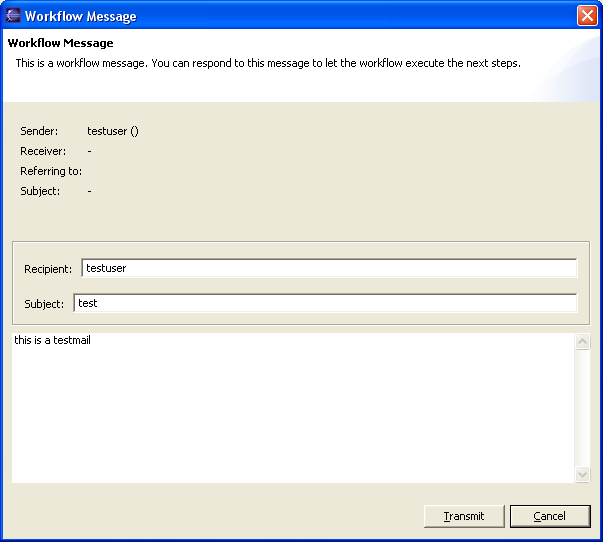
\includegraphics[width=10cm]{tutorial16.png}
   \caption{Write a mail}
\end{center}
\end{figure}\par

Afterwards open the menu of the Workflow View and select 'Fetch messages'. Your sent
message arrives in your Workflow View.

\section{Answering your mail}

In the Workflow View double-click on your testmail. The Workflow
window opens where you can see the message text of the mail. Below you enter
the subject 'reply' and the text of your reply. Send the answer by pressing the 'Transmit' 
button. 

\begin{figure}[h!]
\begin{center}
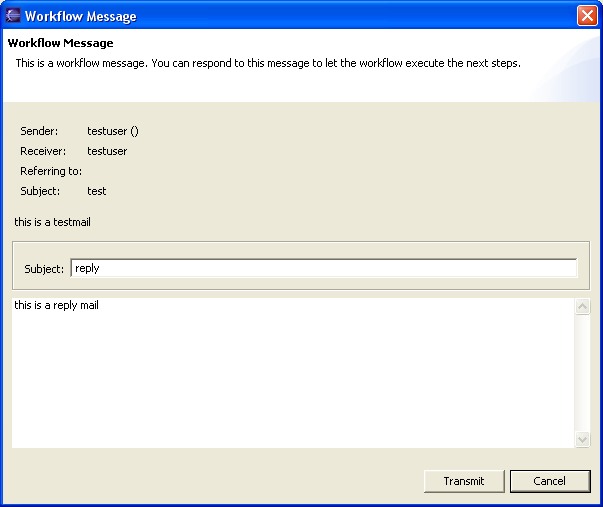
\includegraphics[width=10cm]{tutorial17.png}
   \caption{Answer a mail}
\end{center}
\end{figure}\par

Afterwards open the menu of the Workflow View and select 'Fetch messages'. Your sent
message arrives in your Workflow View.





